\newpage
\section{Using the software}
In this section we will explain by examples how to use the software
for the most common computations. \name consist of a set of subprograms
with names like \texttt{gfan\_bases} and \texttt{gfan\_buchberger} each with
a different purpose. See Appendix \ref{sec:dataformats} for an
explanation of the data formats and Appendix~\ref{sec:applist} for a
full list of the various functions and their help files.

%\emph{In the
%following we will assume that the software has been installed with
%\texttt{make install} and that all subprograms have been installed
%with \texttt{gfan installlinks} - see Section \ref{sec:installation}}.

\subsection{Computing the Gr\"obner fan}
The program \texttt{gfan\_bases} computes the set of reduced Gr\"obner bases
of an ideal. To use it type in the name in the UNIX shell \footnote{It is actually much more convenient to use the Emacs shell. In Emacs press Meta-x and type \textup{shell}. When you are in the Emacs shell Ctrl-up will allow you to easily reinput old polynomial data to \name.}
\begin{verbatim}
gfan_bases
\end{verbatim}
and type in a polynomial ring followed by a set of generators for the ideal
\begin{verbatim}
Q[a,b,c]
{aab-c,bbc-a,cca-b}
\end{verbatim}
For compatibility reasons the polynomial ring can be left out in which case the ring is assumed to be the polynomial ring over the rationals with variable names $a,b,c,\dots$.
The program will output the polynomial ring and the list of
reduced Gr\"obner bases of the input ideal. In this example there are
33 such bases.
% You may want to filter the output through the UNIX
%program \texttt{cat} to separate the debug information and the list of
%Gr\"obner bases. Type the following to do this:
%\begin{verbatim}
%gfan | cat
%\end{verbatim}
%and type in the input as before.

Often it is convenient to store your generators in a text file instead
of typing them in every time you use the program. You can redirect the
standard input for the program to read from a file instead of the
keyboard. For example, if your ring and generators are stored in the file
\texttt{myinputfile.txt} you would type:
\begin{verbatim}
gfan_bases <myinputfile.txt
\end{verbatim}
If you want to store the output in the file \texttt{myoutputfile.txt}
you can redirect the standard output as well:
\begin{verbatim}
gfan_bases <myinputfile.txt >myoutputfile.txt
\end{verbatim}


The list of reduced Gr\"obner bases can be transformed into a polyhedral representation of the Gr\"obner fan by using the program \texttt{gfan\_topolyhedralfan} as explained in Section~\ref{subsec:combining}.

Here is another example of a polynomial ring and an ideal:
\begin{verbatim}
Z/3Z[x_1,x_2,x_3]
{x_1^2x_2-x_3,x_2^2x_3-x_1,x_3^2x_1-x_2}
\end{verbatim}

\subsubsection{Exploiting symmetry}
\label{sec:symmtry}
As explained in Subsection \ref{subsec:global computations} the program can do its computations up to symmetry. In the example above we may cycle the three variables without changing the ideal. Hence the subgroup $G\subseteq S_n$ in Subsection \ref{subsec:global computations} is the group generated by a three cycle. A way to write down the subgroup is by writing a list of permutations that generate the subgroup:
\begin{verbatim}
{(0,1,2),(1,2,0)}
\end{verbatim}
The first permutation is the identity (which can be left out). The second permutation is three-cycle. Together they generate $G$. See Appendix~\ref{sec:dataformats} for more information on how to specify the permutations.

The option \texttt{--symmetry} tells \texttt{gfan} to do its computations up to symmetry. For example,
\begin{verbatim}
gfan_bases --symmetry <anotherinputfile.txt 
\end{verbatim}
will read the generators for the ideal and the generators for the group and perform the computation up to symmetry. The input file would have to look like this:
\begin{verbatim}
Q[a,b,c]
{aab-c,bbc-a,cca-b}
{(0,1,2),(1,2,0)}
\end{verbatim}
The output will be a list of reduced Gr\"obner basis - one for each orbit.

\subsection{Combining the programs}
\label{subsec:combining}
The various \name programs can be combined. For example, if we are interested in the combinatorics of the Gr\"obner fan rather than the Gr\"obner bases, we can run the command:
\begin{verbatim}
gfan_bases <myinputfile.txt | gfan_topolyhedralfan
\end{verbatim}
The output is a polyhedral fan in the format explained in Appendix~\ref{format:fan}.

Similarly, the command line
\begin{verbatim}
gfan_buchberger <myinputfile.txt | gfan_groebnercone
\end{verbatim}
produces the polyhedral cone (Appendix~\ref{format:cone}) of the computed reduced Gr\"obner basis, and
\begin{verbatim}
gfan_buchberger <myinputfile.txt | gfan_groebnercone --asfan
\end{verbatim}
computes the cone as a polyhedral fan (Appendix~\ref{format:fan}) with all faces of the cone listed.

As another example, if we are interested in the list of monomial initial ideals rather than the complete list of reduced Gr\"obner bases of an ideal we will pipe the output of \texttt{gfan\_bases} through the program \texttt{gfan\_leadingterms}:
\begin{verbatim}
gfan_bases <myinputfile.txt | gfan_leadingterms -m
\end{verbatim}
%or if we want to direct the output:
%\begin{verbatim}
%gfan <myinputfile.txt | gfan_leadingterms -m >myoutputfile.txt
%\end{verbatim}
We need to use the option \texttt{-m} to tell \texttt{gfan\_leadingterms} that it should expect a list of Gr\"obner bases rather than a single Gr\"obner basis on its input.

If we want the union of the Gr\"obner bases instead we should type:
\begin{verbatim}
gfan_bases <myinputfile.txt | gfan_polynomialsetunion >myoutputfile.txt
\end{verbatim}
This will compute a \emph{universal Gr\"obner basis}.

In three variables, if we want to draw staircase diagrams of the initial ideals we may use the program \texttt{gfan\_renderstaircase}:
\begin{verbatim}
gfan_bases --symmetry <anotherinputfile.txt | 
                        gfan_renderstaircase -m -w6 -d16 >out.fig
\end{verbatim}
The output file is the xfig file in Figure \ref{fig:staircase}. To save paper we used the \texttt{--symmetry} option and gave the program the file also containing the group generators as input.
\begin{figure}
\begin{center}
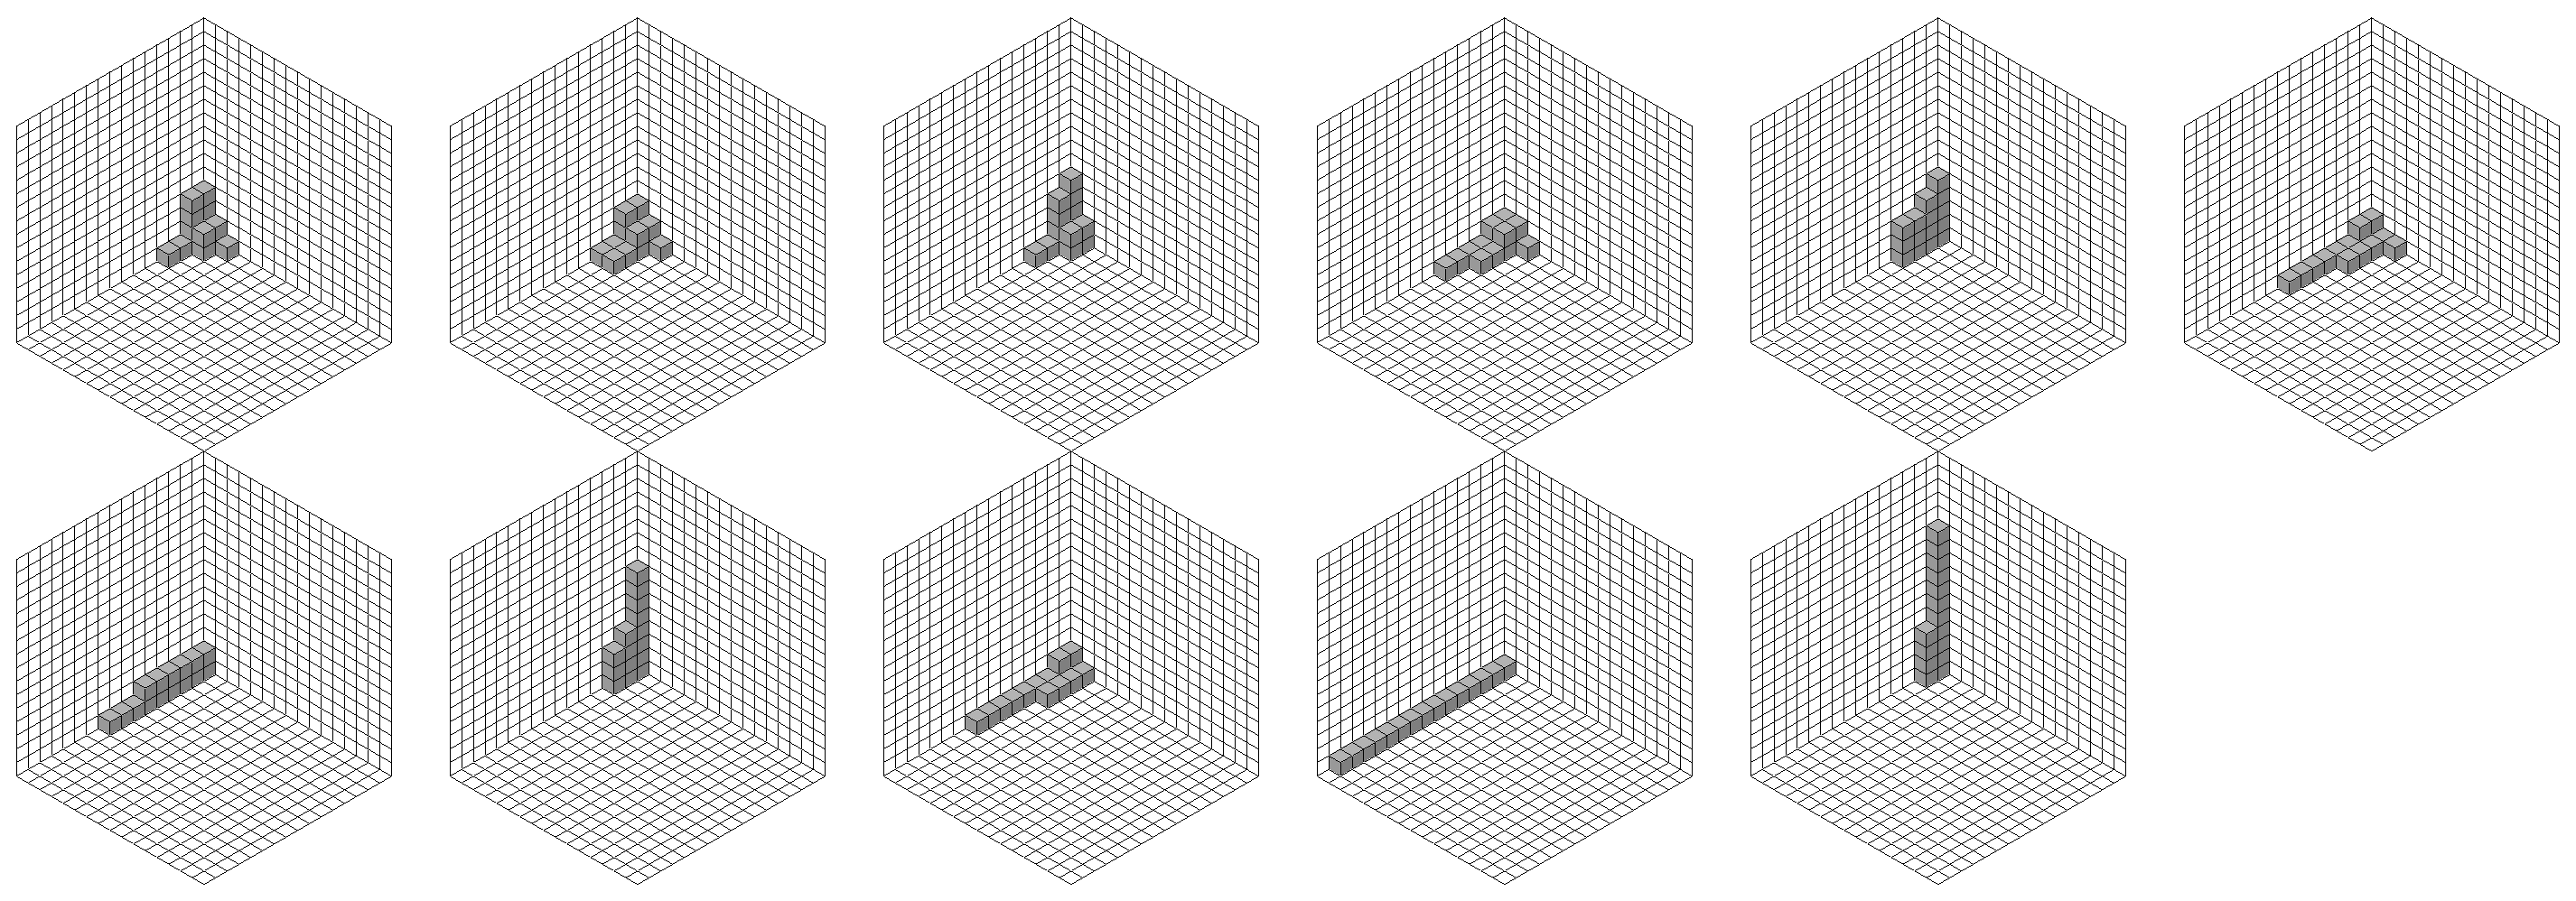
\epsfig{file=staircase.eps,height=4.5cm} 
\end{center}
\caption{Staircase diagrams of the monomial initial ideals in the example - up to symmetry.}
\label{fig:staircase}
\end{figure}
 

In three variables, if we want to draw the Gr\"obner fan - or rather draw the intersection of the $2$-dimensional standard simplex with the Gr\"obner fan we may use the program \texttt{gfan\_render}:
\begin{verbatim}
gfan_bases <myinputfile.txt | gfan_render >myoutputfile.fig
\end{verbatim}
The output is shown in Figure \ref{fig:gfan}.
If there are more than three variables in the polynomial ring this program can still be used but it is more difficult. See Appendix~\ref{applist:_render}.
\begin{figure}
\begin{center}

\epsfig{file=gfan.eps,height=5.9cm} 
\end{center}
\caption{The Gr\"obner fan of the ideal intersected with the standard simplex.}
\label{fig:gfan}
\end{figure}

\subsection{Interactive mode}
To study the local structure of the Gr\"obner fan the program \texttt{gfan\_interactive} is useful. It allows the user to walk along an arbitrary path of full dimensional Gr\"obner cones in the Gr\"obner fan of the ideal. At each step the user will specify which facet to walk through. The input must be a marked Gr\"obner basis. The program will minimise and autoreduce if necessary to get the reduced Gr\"obner basis. For example running the program
\begin{verbatim}
gfan_interactive
\end{verbatim}
with input
\begin{verbatim}
Q[a,b,c]
{
c^15-c,
b-c^11,
a-c^9}
\end{verbatim}
will give us a list of facets to walk through. (One way to get a starting Gr\"obner basis is by using the program \texttt{gfan\_buchberger}.) In this case only two flips are possible, since the third wall does not lead to a new Gr\"obner cone. -- The wall is on the boundary of the Gr\"obner region. We may choose any of the two remaining facets by typing in an index (a number) followed by $<$ enter $>$. See Appendix \ref{applist:_interactive} for more options.
%\subsection{Other useful programs}
%We list a few more interesting programs in the package. The remaining programs can be found in Appendix \ref{sec:applist}.
%\subsubsection{Computing a Gr\"obner cone}
%The program \texttt{gfan\_groebnercone} extracts a defining set of half-spaces for a Gr\"obner cone.
%The input is a Gr\"obner basis for the cone. The output is a list of vectors - each specifying a half-space.
%For example we may compute the restricted Gr\"obner cone of the lexicographic basis above by running
%\begin{verbatim}
%gfan_groebnercone --restrict
%\end{verbatim}
%with the reduced Gr\"obner basis as input.
%
%\subsubsection{Computing the facets of a Gr\"obner cone}
%The program \texttt{gfan\_facets} will take a list of vectors - each specifying a half-space whose intersection is a full-dimensional cone and compute a minimal set of defining half-spaces for the cone. Thus, we can compute the inner facet normals of the Gr\"obner cone above by running
%\begin{verbatim}
%gfan_groebnercone --restrict | gfan_facets
%\end{verbatim}
%with the reduced Gr\"obner basis as input.
%
%\subsubsection{Computing a weight vector}
%The program \texttt{gfan\_weightvector} will compute a strictly positive interior point of a Gr\"obner cone given by its reduced Gr\"obner basis. In our example, if we run
%\begin{verbatim}
%gfan_weightvector
%\end{verbatim}
%on the lexicographic basis we (might) get the vector
%\begin{verbatim}
%(21,25,2)
%\end{verbatim}


\subsection{Integers and p-adics}
Gfan handles two settings in which the usual division and Buchberger algorithms do not suffice. These are ideals in $\Z[x_1,\dots,x_n]$ and $\Q[x_1,\dots,x_n]$, where, in the latter setting, the $p$-adic valuation is taken into account when defining initial ideals.

At the moment these two settings are handled by the commands \texttt{gfan\_overintegers} and \texttt{gfan\_padic}. They allow the computation of Gr\"obner bases, initial ideals, Gr\"obner cones (or polyhedra) and Gr\"obner fans (or complexes). In this section we give two examples. Use the \texttt{--help} option to get the full documentation.

\begin{example}
To compute the Gr\"obner fan of \cite[Example~3.9]{sturmfels}, with the ideal considered in the ring $\Z[a,b,c]$ we run the command
\begin{verbatim}
gfan_overintegers --groebnerFan -g --log1
\end{verbatim}
on
\begin{verbatim}
Q[a,b,c]
{a^5+b^3+c^2-1, b^2+a^2+c-1, c^3+a^6+b^5-1}
\end{verbatim}
Since the type-system of Gfan does not understand {\texttt Z[a,b,c]} we need to trick Gfan by specifying the ring $Q[a,b,c]$ when running {\texttt gfan\_overintegers}. From the output we conclude that the ideal has $1659$ reduced Gr\"obner bases over the integers (as opposed to $360$ over a field of characteristic $0$).
\end{example}

\begin{example}
To compute the reduced Gr\"obner basis of $I=\langle x_1+2x_2-3x_3, 3x_2-4x_3+5x_4\rangle\subseteq \Q[x_1,\dots,x_4]$ with respect to the vector $(1,0,0,1)$ (tie-broken lexicographically) and with $\Q$ having the $2$-adic valuation,
we run
\begin{verbatim}
gfan_padic --groebnerBasis -p2
\end{verbatim}
on the input
\begin{verbatim}
Q[x1,x2,x3,x4]
{
x1+2x2-3x3,
3x2-4x3+5x4
}
(1,1,0,0,1)
\end{verbatim}
The first coordinate of the input vector is a $1$, since {\texttt \_padic} requires ``homogenized'' weight vectors. This is Example 2.4.3 in the upcoming book by Maclagan and Sturmfels on tropical geometry. The division algorithm implemented in Gfan used for this computation was proposed by Maclagan. To find all initial ideals, we can use a combination of \texttt{gfan\_padic --groebnerBasis}, \texttt{gfan\_combinerays --section CONES -i filename} and \texttt{gfan\_padic --initialIdeals -m}.

Notice that the Gr\"obner complex of $I$, where valuation is taken into account (see Maclagan-Sturmfels), is not a fan. The output of \texttt{gfan\_groebnerComlex}, however, will be a fan. To get the Gr\"obner complex we need to intersect the fan with the hyperplane $\omega_0=1$.

NOTICE THAT \texttt{\_padic} USES THE MINIMUM CONVENTION AT THE MOMENT - in order to be consistent with Maclagan and Sturmfels.
\end{example}


\subsection{Toric ideals and secondary fans}

Gfan is a replacement of the software CaTS \cite{cats} which computes Gr\"obner fans of toric and lattice ideals.
For convenience a program for computing lattice ideals has been added to Gfan.
To compute the lattice ideal of the lattice generated by $(2,-1,0)$ and $(3,0,-1)$ we run:
\begin{verbatim}
gfan_latticeideal
{(2,-1,0),(3,0,-1)}
\end{verbatim}
Gfan will transform the generators into binomials and compute the
saturation of the ideal they generate by the product of all variables. The computation is independent of the characteristic of the field.

If on the other hand we wish to compute the toric ideal of a \emph{vector configuration} given by the columns of the $1\times 3$-matrix $(1,2,3)$ we run
\begin{verbatim}
gfan_latticeideal -t
{(1,2,3)}
\end{verbatim}
More rows can be added to the matrix if we want.

The choice of the term ``vector configuration'' is intentional and nonstandard. The reason for this will become clear later in this section. In Gfan terminology a \emph{point configuration} is reserved for the collection of points we have before we add a row of ones to construct a projective toric variety. By adding the row of ones the point configuration is turned into a vector configuration.
Notice that scaling a vector of a vector configuration may change its toric ideal.

Computing toric ideals Gfan is not optimal. If one needs to do big examples the software 4ti2 \cite{4ti2} is recommended.

For a toric ideal the radical of a monomial initial ideal is the Stanley-Reisner ideal of a regular triangulation of the point configuration, see \cite{sturmfels}. Hence the toric Groebner fan is a refinement of the \emph{secondary fan}, indexing all regular triangulation of the point configuration.

The secondary fan of the vector configuration $\{(1,0),(1,1),(1,2),(1,3)\}$ can be computed by typing
\begin{verbatim}
gfan_secondaryfan
{(1,0),(1,1),(1,2),(1,3)}
\end{verbatim}
Comparing this to the finer Gr\"obner fan of the corresponding toric ideal which you get by doing
\begin{footnotesize}
\begin{verbatim}
gfan_transposematrix  | gfan_latticeideal -t | gfan_bases | gfan_topolyhedralfan 
{(1,0),(1,1),(1,2),(1,3)}
\end{verbatim}
\end{footnotesize}
you realise that three monomial initial ideals of the toric ideal have the same radical, while four monomial initial ideals pairwise have the same radical.

The secondary fan computation was added for convenience.
%For any
%serious computation with secondary fans you should use
An alternative is to use
TOPCOM \cite{rambau}.  Notice however, that the vector configurations
for gfan\_secondaryfan do not have to be pointed. This means that
all combinatorial types of polytopes with a fixed set of normals can
be easily enumerated. This is not possible with TOPCOM.
